%% This is emulateapj reformatting of the AASTEX sample document
%%
\documentclass{emulateapj}
\usepackage{amsmath}

%% You can insert a short comment on the title page using the command below.

%\slugcomment{Report for Independent Research}

%% If you wish, you may supply running head information, although
%% this information may be modified by the editorial offices.
%% The left head contains a list of authors,
%% usually a maximum of three (otherwise use et al.).  The right
%% head is a modified title of up to roughly 44 characters.
%% Running heads will not print in the manuscript style.

\shorttitle{Determination of Kinematic Inclinations}
\shortauthors{Beauchemin}

%% This is the end of the preamble.  Indicate the beginning of the
%% paper itself with \begin{document}.

\begin{document}

%% LaTeX will automatically break titles if they run longer than
%% one line. However, you may use \\ to force a line break if
%% you desire.

\title{Determining Galaxy Inclinations from Kinematics}

%% Use \author, \affil, and the \and command to format
%% author and affiliation information.
%% Note that \email has replaced the old \authoremail command
%% from AASTeX v4.0. You can use \email to mark an email address
%% anywhere in the paper, not just in the front matter.
%% As in the title, use \\ to force line breaks.

\author{Ryan Beauchemin, Sheila Kannappan, Charlie Bonfield}
\affil{Department of Physics and Astronomy, University of North Carolina at Chapel Hill}
%\email{rwbeauchemin@unc.edu}

%\author{Names of second author -- delete if not relevant}
%\affil{Astronomy Department, University of Florida, Gainesville, FL 32611}

%\and

%\author{Name of Third author -- delete if not relevant}
%\affil{Space Telescope Science Institute, Baltimore, MD 21218}


%% Mark off your abstract in the ``abstract'' environment. In the manuscript
%% style, abstract will output a Received/Accepted line after the
%% title and affiliation information. No date will appear since the author
%% does not have this information. The dates will be filled in by the
%% editorial office after submission.

\begin{abstract}
The distribution of inclinations of spiral galaxies in any area in the sky is expected to be completely random in an isotropic universe. Surprisingly, we find that this is not the case when using inclinations determined from the projected shape of the galaxy or photometric inclinations. We have compared photometric inclinations with kinematic inclinations, which are derived from the distribution of Doppler shifted velocities in the galaxy as measured by the 4.1m SOAR telescope and Goodman spectrograph. We also compare results from two different codes for measuring kinematic inclinations. The first code is called DiskFit, and it takes a number of points in discrete elliptical annuli and fits based on the averages of velocities within those annuli. The second is one that we developed that uses all data points simultaneously, called Velocity Field Fitter (VFF). We quantify the differences between the two fitting methods to determine the success of their application as a function of galaxy size and shape. 
\end{abstract}

%---------------------------------------------------------------------------------%
%                             Section 1: Introduction                             %
%---------------------------------------------------------------------------------%

\section{Introduction}
\subsection{The RESOLVE Survey}
In the UNC-led REsolved Spectroscopy Of a Local VolumE (RESOLVE) survey, all galaxies in a nearby volume are observed regardless of size or luminosity in what is considered to be a volume-limited fashion. This is much more statistically representative of the composition of our universe on a larger scale than the classical approach that is limited by apparent brightness, where one obtains data for only the brightest galaxies, ones which are not very common in the universe. Though these surveys give us a good idea about the large scale structure of the universe, it is also pertinent to our understanding of the universe that we explore the small scale details that make this up. The RESOLVE team members at UNC are well-situated to observe local environments because UNC, as a partner, is guaranteed a portion of time every year and competes nationally for more time on the 4.1 meter SOAR telescope, which has been erected in Chile and is capable of taking highly-resolved (0.22 arc seconds per pixel) spectra of galaxies. With the large number of observed galaxies in the RESOLVE survey, we can determine how photometric properties might change in the RESOLVE survey with the expectation that most of them should be random in the volume-limited sample. When examined, the distribution of photometric inclinations were not as expected.

\subsection{Photometric Inclination}

Inclinations are defined as the projected tilt of a disk galaxy ranging from 0 to 90 degrees, or from face-on to edge-on. We have analyzed the galaxies photometrically, using the axial ratio of the projected ellipse to determine its inclination by the classic formula from \citet{hubble}

\begin{equation}
i = cos^{-1}(((q^2-q_0^2)/(1-q_0^2))^{1/2})
\end{equation}

\noindent where $q$ is the major to minor axial ratio and $q_0$ is the ratio at an inclination of 90 degrees. Since disk galaxies are not flat, $q_0$ must be greater than 0, and is taken to be 0.2, as determined by \citet{holmberg}. We find that the distribution of photometrically determined inclinations for disk galaxies is not random, as can be seen in Figure 1.

\begin{figure}
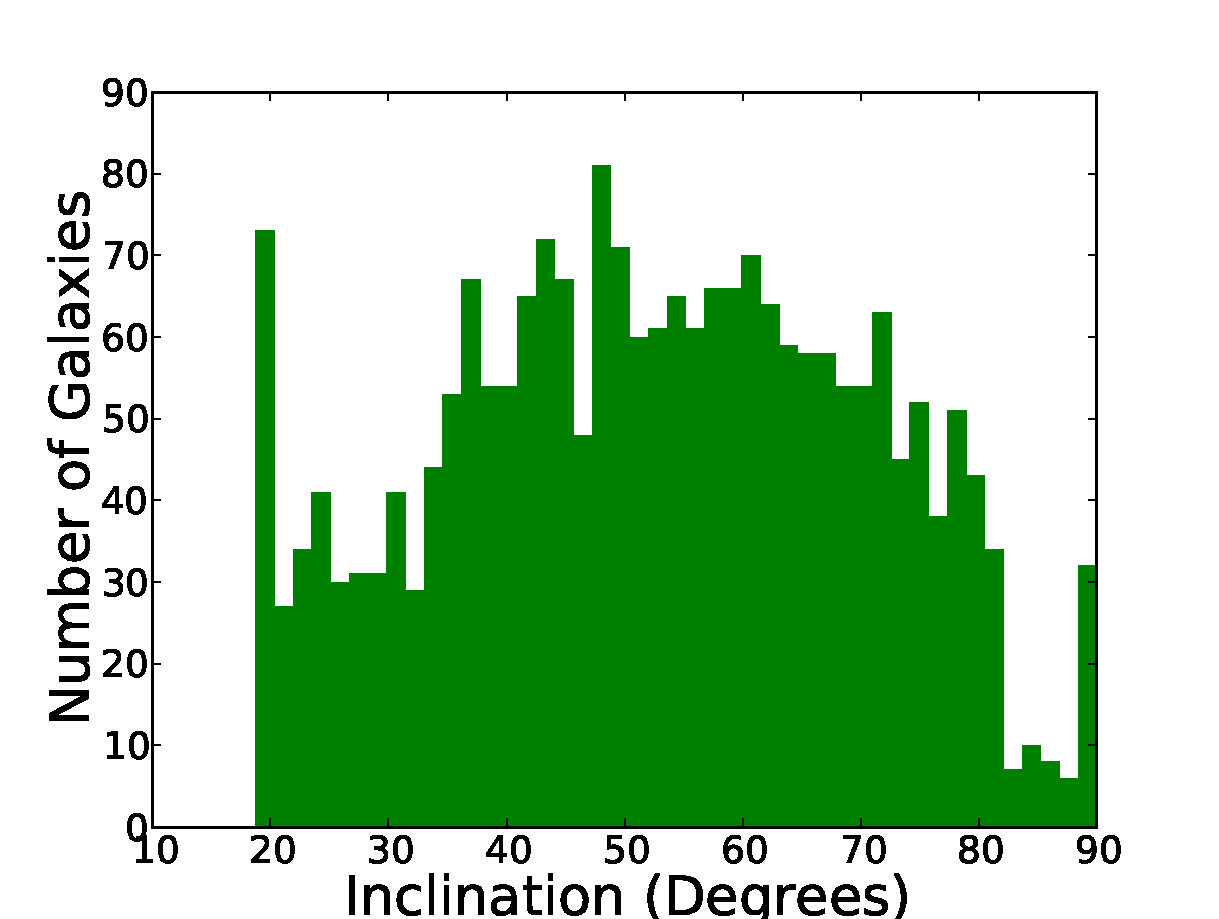
\includegraphics[width=0.5\textwidth]{hist1.pdf}
\caption{The distribution of photometric inclinations in the RESOLVE survey. If the measurement was truly random, this distribution should be fairly flat. \label{fig:test}}
\end{figure}

We are interested in finding why this is the case, since we would expect there to be no preference in a volume-limited survey. The root of this problem may lie in either the way that photometric inclinations are calculated or in our understanding of the intrinsic shapes of disk galaxies. I have been working towards ruling out one of these options in answering the question: Is our current method of photometric inclination determination sound, and if not, what photometric properties cause this error? This is an important question to tackle because galactic astronomers have for almost a century been using a simple equation which assumes a lot about the shape and structure of a galaxy, and has not yet been tested vigorously for robustness. Luckily, there is another way to determine the inclination of galaxies that assumes much less about the structure.

%%%%%%%%%%%%%%%%%%%%%%%%%%%%%%%%%%%%%%%%%%%%%%%%%%%%%%%%%%%%%%%%%%%%%%%%%%%%%%%%%%%
%%%%%%%%%%%%%%%%%%%%%%%%%%%%% YOU STOPPED HERE LAST %%%%%%%%%%%%%%%%%%%%%%%%%%%%%%%
%%%%%%%%%%%%%%%%%%%%%%%%%%%%%%%%%%%%%%%%%%%%%%%%%%%%%%%%%%%%%%%%%%%%%%%%%%%%%%%%%%%

\subsection{Kinematic Inclination}

Kinematic inclinations are inclinations found from the observed velocity fields of spiral galaxies. These galaxies are rotating about a central point, and the line-of-sight velocities from Doppler shifting can be detected by a spectrograph to determine the average velocities of baryonic matter in the line of sight. Using the maximum velocity calculated from luminosity as described by \citet{tullyfish}, one may determine how far from edge-on a galaxy is. This can be done because an observed edge-on galaxy would have almost all of its velocity in the line of sight, whereas a face-on galaxy would show only the cosmological redshift at most of the points in the galaxy. One may model the continuum of possible inclinations based on the velocity fields. This can be seen in the equation relating projected velocities with inherent velocities described by \citet{teuben}

\begin{equation}
V = V_{sys}+V_{rot}(R)\cos{\theta}\sin{i} + V_{exp}(R)\sin{\theta}\sin{i}
\end{equation}

\noindent where $\theta$ is the angle of the deprojected galaxy, and $i$ is the inclination from (1). We believe that the kinematic method of inclination measurement is more accurate because it makes less assumptions about the intrinsic properties of a spiral galaxy. There are processes which can tidally disturb the velocities in some regions of galaxies, but the effects appear to be minimal when determining the inclination on a larger scale. With two different ways of measuring inclination, we have made a comparison of measurements using the two methods and how their differences relate to other properties of galaxies to see where these differences might come from. With the belief that the kinematic method provides a more accurate representation of a galaxy's true inclination, this also means that we might expose faults in the measurement of photometric inclinations. 


%---------------------------------------------------------------------------------%
%                                  Section 2: Data                                %
%---------------------------------------------------------------------------------%

\begin{figure}
%\plotone{rf0071example.pdf}
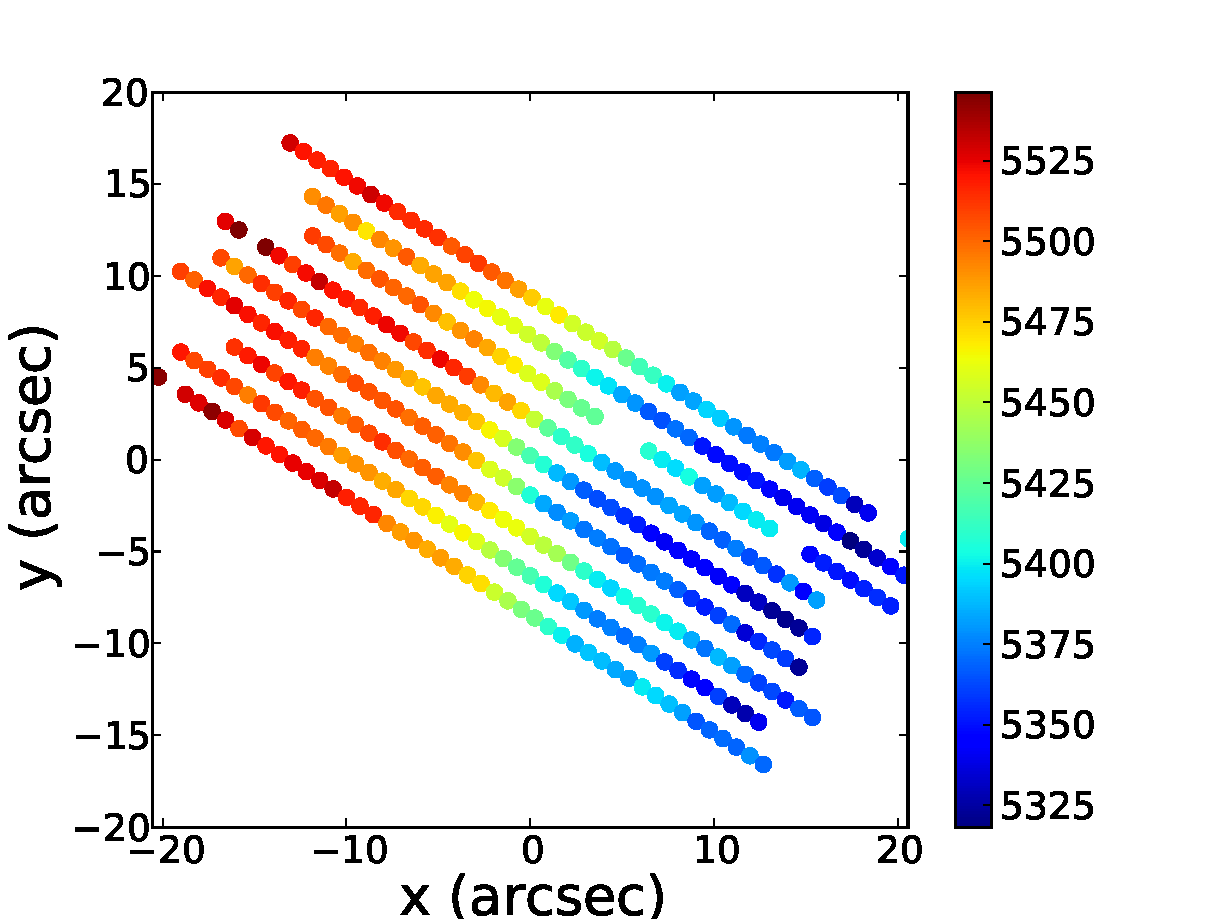
\includegraphics[width=0.5\textwidth]{rf0071example.pdf}
\caption{An example of the velocity field of a nearly face-on galaxy with three pointings from the fall catalog of the RESOLVE survey, with velocities given in km/s. \label{fig:test}}
\end{figure}


\section{Data}

\begin{figure}
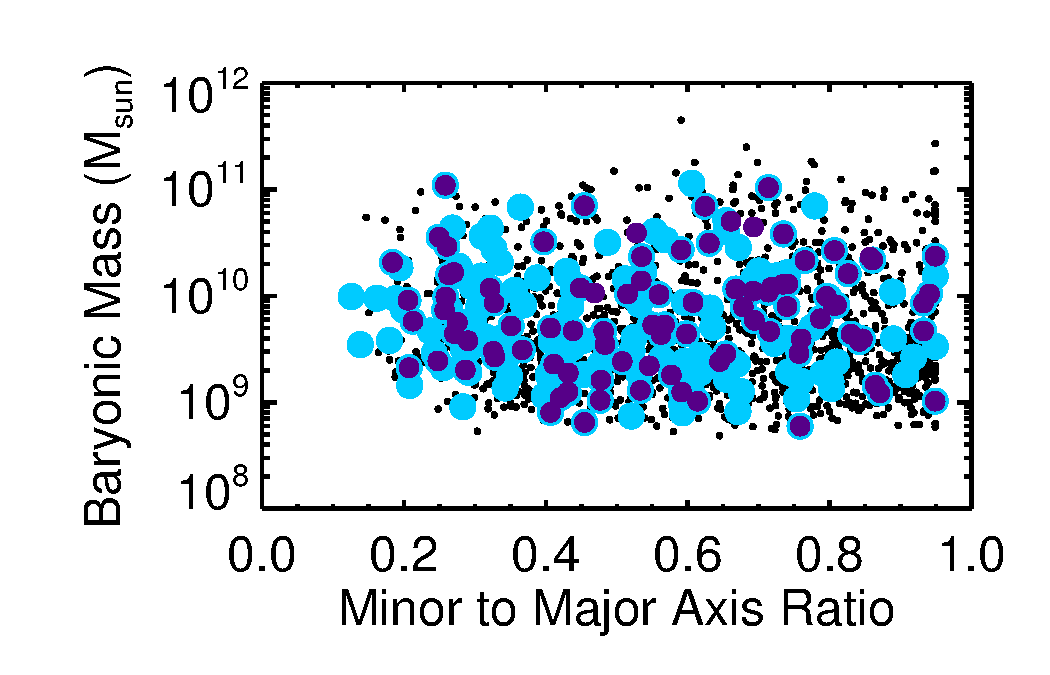
\includegraphics[width=0.5\textwidth]{naxisratio-eps-converted-to.pdf}
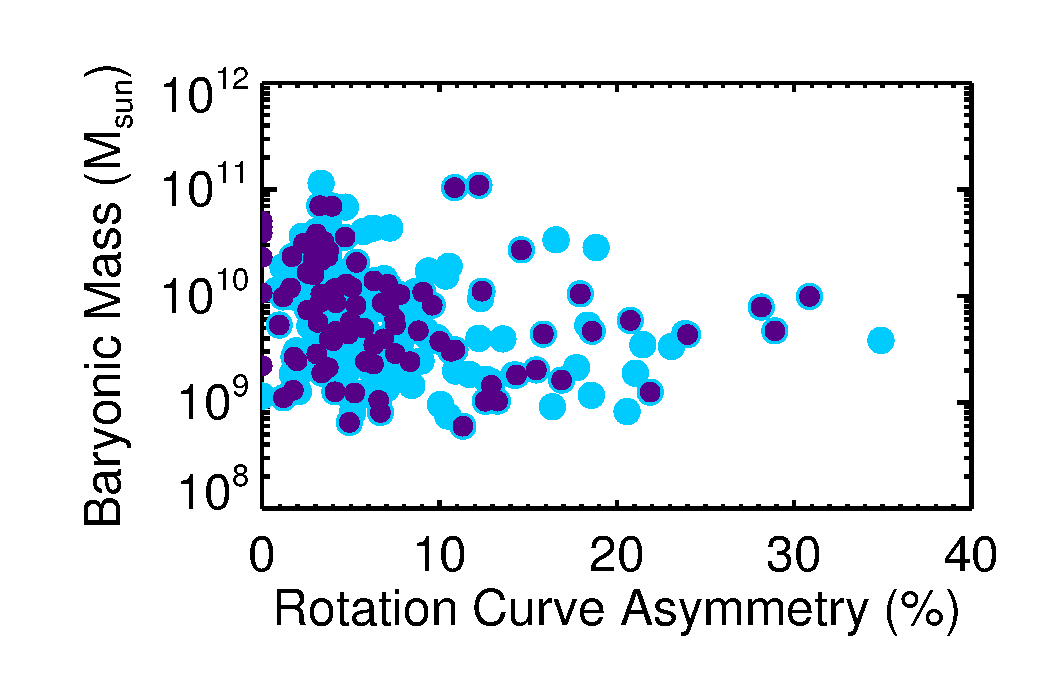
\includegraphics[width=0.5\textwidth]{nasymHa-eps-converted-to.pdf}
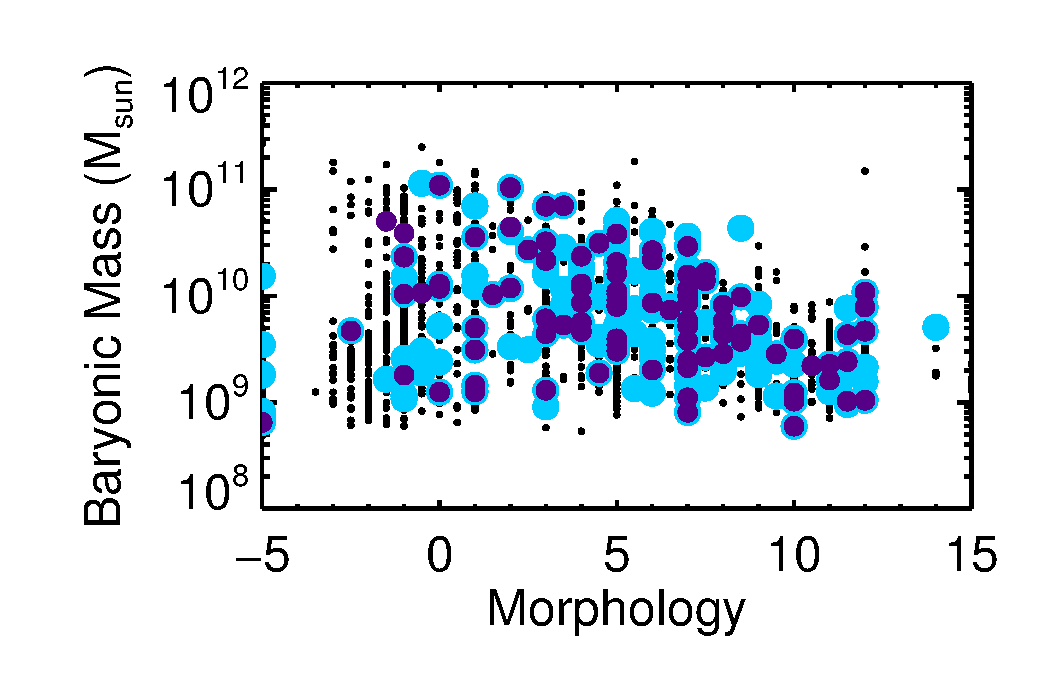
\includegraphics[width=0.5\textwidth]{nmorph-eps-converted-to.pdf}
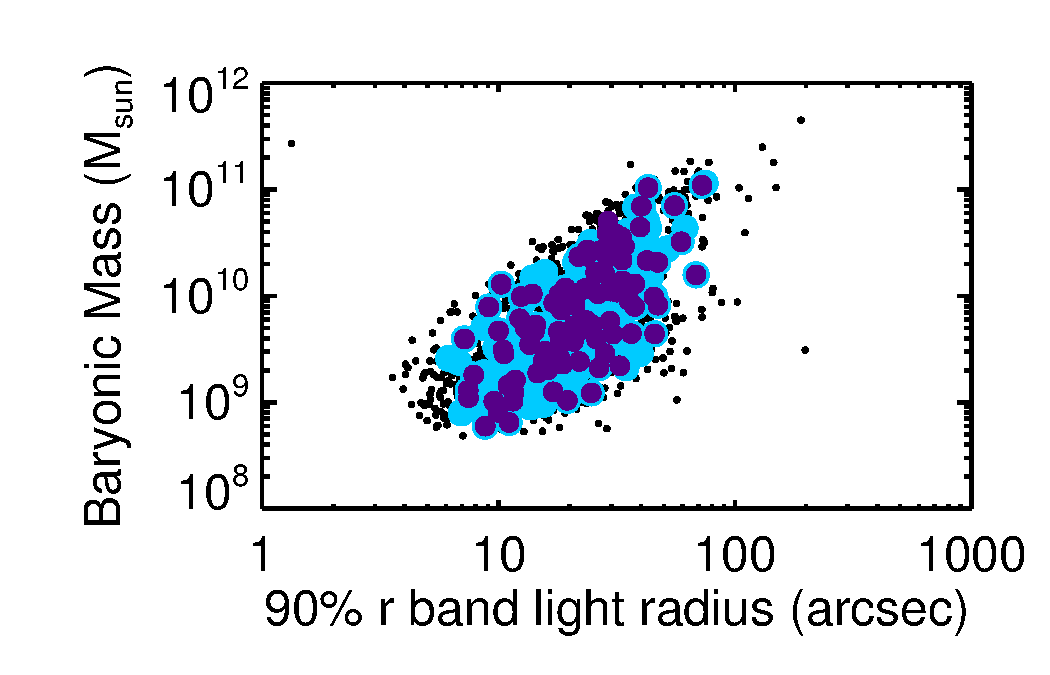
\includegraphics[width=0.5\textwidth]{nradr90p-eps-converted-to.pdf}

\includegraphics[width=0.5\textwidth]{stuff-Recovered-eps-converted-to.pdf}
\caption{Baryonic mass against axial ratio, rotation curve asymmetry, morphology, and 90\% r band light radius. \label{fig:test}}
\end{figure}

We observe galaxies using the 4.1m SOAR telescope and collect spectra using it's GOODMAN spectrograph with a custom-built spectrograph image slicer that allows up to three nearby spectra to be taken at once without overlap. All data is reduced through a pipeline created by the RESOLVE team. Of the galaxies in the survey, a subsample including all previously reduced data was selected for the comparison of photometric and kinematic inclinations. To ensure that the sample was representative of the larger survey, we checked various properties of interest based on what we would expect might have an effect on the two dimensional projection of a galaxy and what might have an effect on the observed velocity field, which would in turn affect the photometric and kinematic inclination measurements respectively. Properties that we decided would have an effect are the galaxy's morphology, rotation curve asymmetry, and radius at which 90 percent of the galaxy's r-band light is contained within. For statistical reasons, we also made sure to have a representative distribution of all the axial ratios found within the survey.


%---------------------------------------------------------------------------------%
%                           Section 3: Kinematic Vfitting                         %
%---------------------------------------------------------------------------------%

\section{Kinematic Velocity Fitting Methods}

\subsection{DiskFit}

A publicly available code called DiskFit \citep{barnes} is capable of fitting the velocity field data that we have to a model profile given initial guesses to the position angle and galaxy center. Using DiskFit to model velocity fields for $\sim$100 galaxies, we have found there to be no clear link between the differences in inclination measurements and galaxy properties such as total baryonic mass, rotation curve asymmetry, 90\% r-band radii, or morphology, but we did find some problems fitting small, asymmetric, or barred structures in the disk-fitting algorithm. This makes sense because the model requires many points in order to fit at many annuli and the program assumes the rotation curve to be inherently smooth, but perturbations might easily be misinterpreted, especially with the weight they would have in a small annulus.

\subsection{Velocity Field Fitting}

To remedy this, we have created a new algorithm that uses all of the data simultaneously, without the necessity of fitting disk annuli to it. We first find the center of kinematic rotation in the Doppler velocity field, then we use equations from \citet{teuben} that provide a translation from projected velocities to rotational velocities. Next, we map out the rotation curve of the galaxy and fit the rotation curve to the functions described by \citet{courteau} using minimum chi squared minimization techniques described by \citet{mpfit} in Python. We have found that there is a distinct advantage in doing this for small galaxies that do not have enough data in each annulus to make a clear disk but still have enough information to give a reasonable kinematic profile. So far, we have found that kinematic inclinations are more random than their photometric counterparts, but we still have not compared the differences with other photometric properties, as we did before with the DiskFit models.

%---------------------------------------------------------------------------------%
%                                Section 4: Results                               %
%---------------------------------------------------------------------------------%

\section{Results}
We employed various tests on VFF to see whether it holds up well to different problems in fitting velocity fields. Most of these tests involve making a perfect profile, introducing effects, then re-examining the ability for the code to recognize the original profile.
\subsection{Perfect Fields}
As a zeroth order test, we made sure that the re-examination of a perfect field gave exactly the right inclination, and the correlation was a perfect one-to-one for well-sampled fields with no turbulence or other large perturbations in the field. DiskFit performed just as well in this test.

\begin{figure}[h]
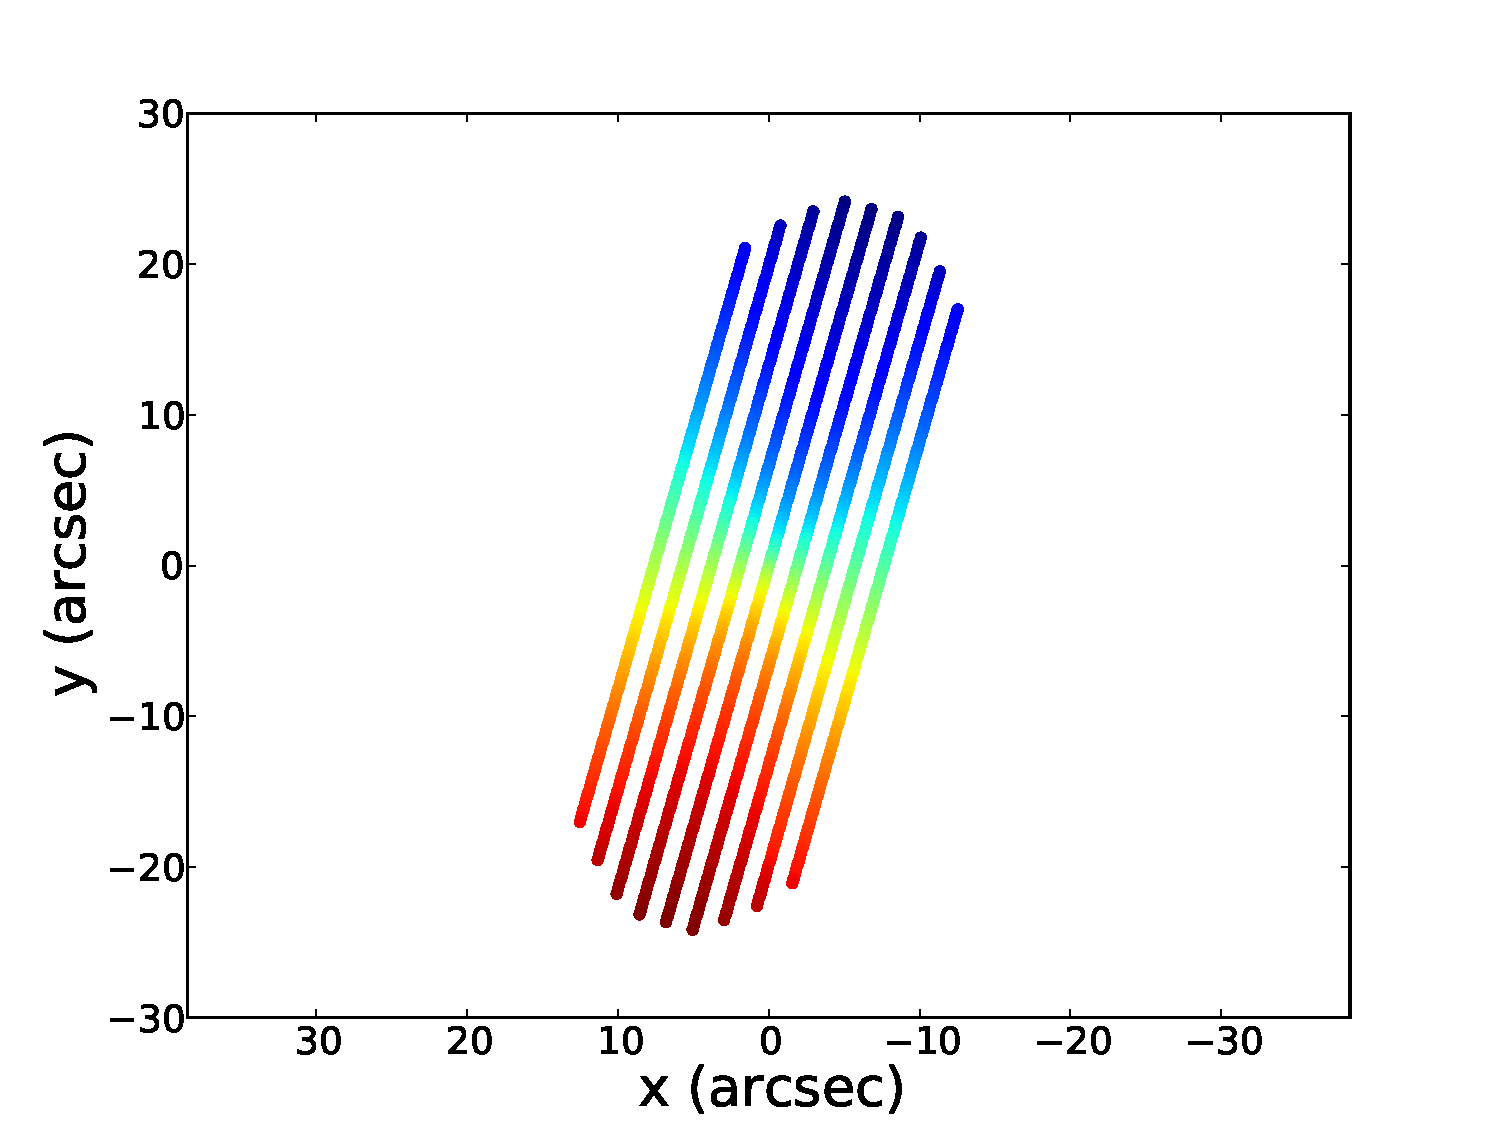
\includegraphics[width=0.5\textwidth]{perfectexamp.pdf}
\caption{An example of a velocity field generated to perfectly fit the photometrically determined properties of a galaxy in the sample with three pointings. \label{fig:test}}
\end{figure}

\subsection{Fields with Turbulence}
Next, we introduced random Gaussian noise across the perfect velocity field to model turbulence. The re-examination for 60, 120, and 200 km/s yielded a one-to-one correlation with the original dataset. HOW DOES VFF PERFORM VS DISKFIT? PLOT IT
%%%%%%% MAKE CHANGES HERE %%%%%%%%


\begin{figure}[h]
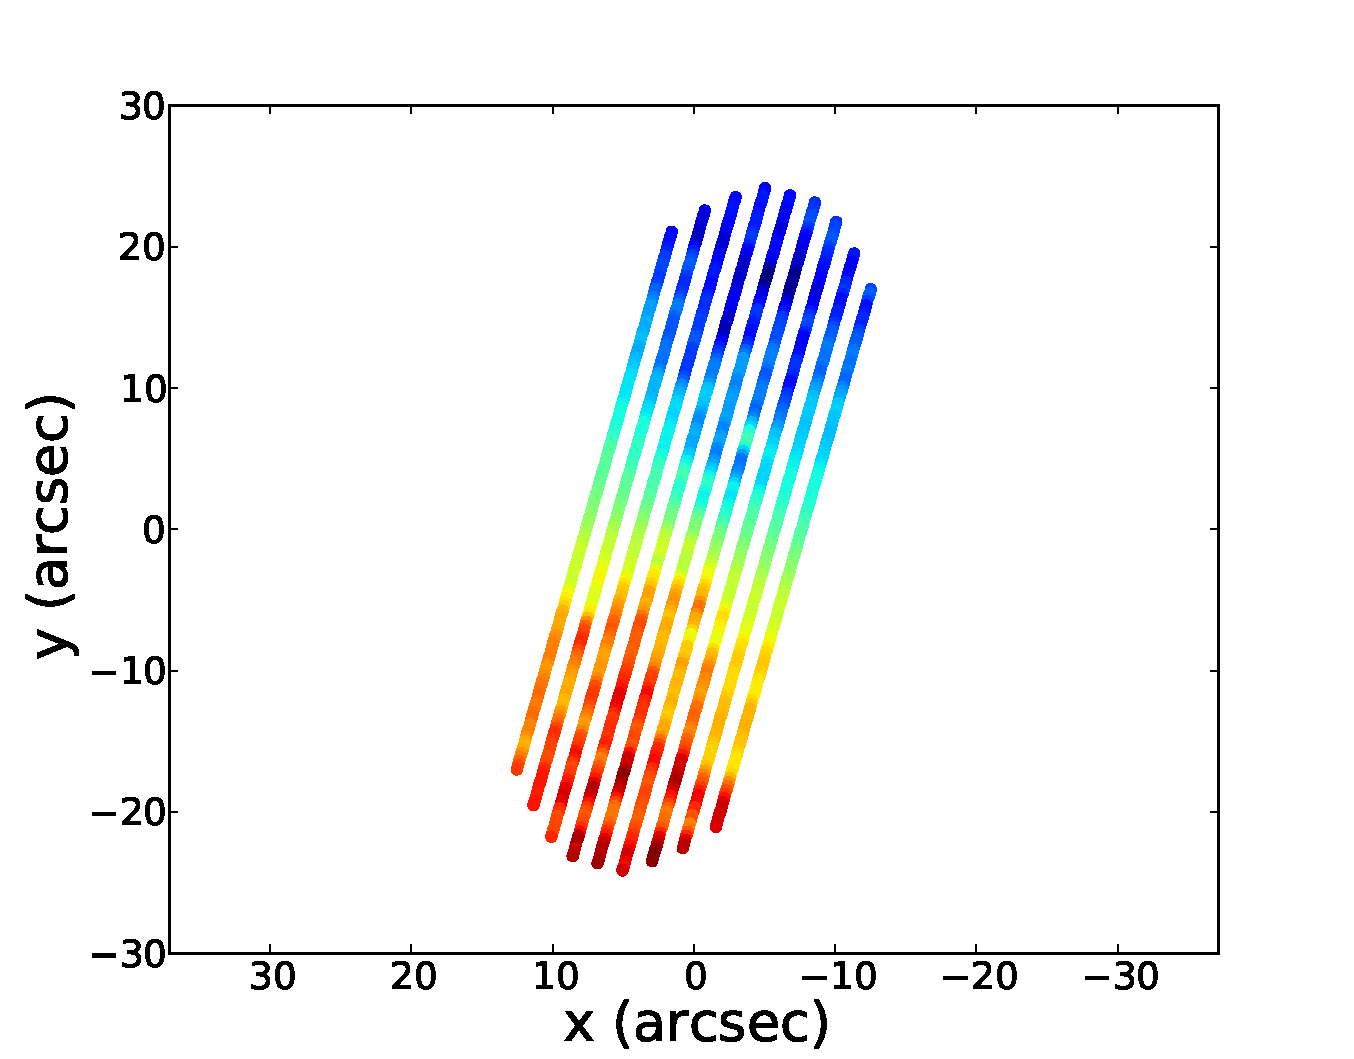
\includegraphics[width=0.5\textwidth]{turbexamp.pdf}
\caption{The same field from Figure 4, but with 120 km/s Gaussian noise added to the velocity. This models the effects of dust and atmosphere missed by the ADC.  \label{fig:test}}
\end{figure}

\begin{figure}[h]
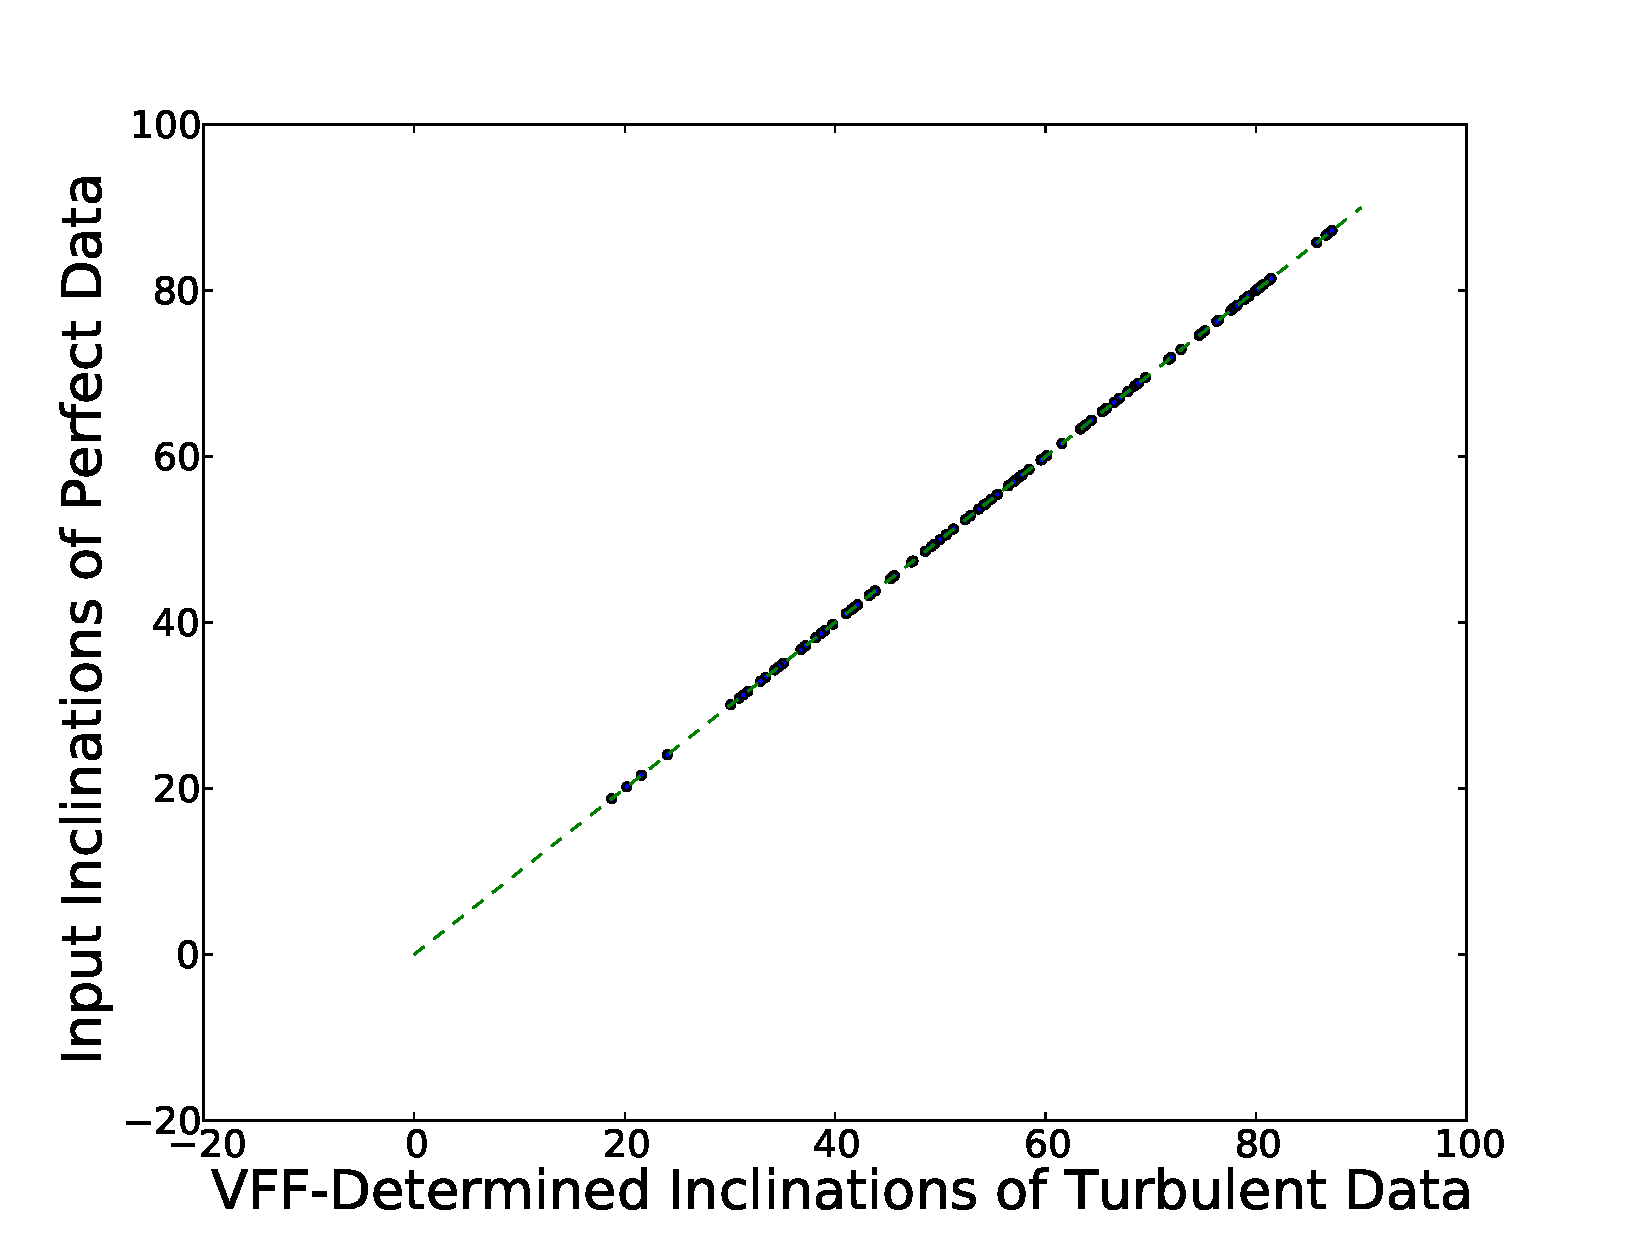
\includegraphics[width=0.5\textwidth]{turbtest.pdf}
\caption{The one-to-one correlation with input parameters and output parameters from VFF after 60 km/s turbulence was added. \label{fig:test}}
\end{figure}

\subsection{Binned Down Perfect Fields}
This test attempted to determine how the fitting process holds up against binned down data from the perfect fields to simulate the resolution of a realistic observation of a galaxy. In fact, for each galaxy we binned at the locations of the actual data from the RESOLVE survey, and used the distance between it and its nearest neighbor as the binning radius. This test gave DiskFit a lot of trouble, making half of the galaxies fail the Fortran fitting procedure that it employs (BRENT). VFF fit all of the galaxies that this test included, but it did not give a one-to-one correlation to the original properties, and fit on average to a lower inclination than the input. This effect is still being investigated in regards to a possible problem with longslit data, but it is promising that the routine does not give up so easily as DiskFit.
%%%%%% WRITE FINDINGS FROM CHECKING THIS!!! %%%%%%%%%
\begin{figure}[h]
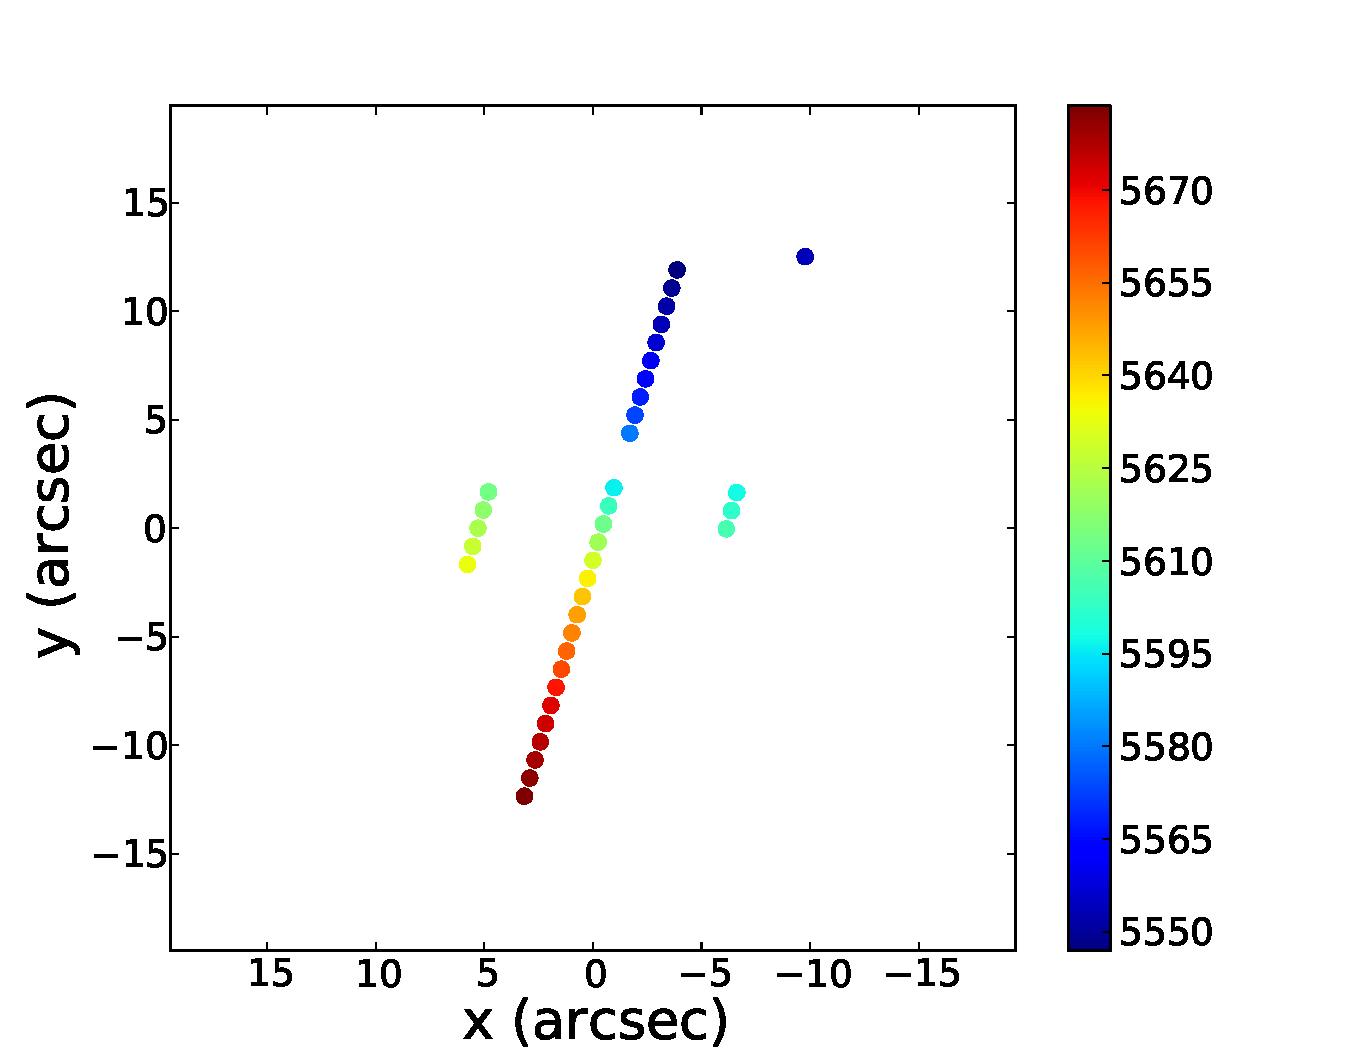
\includegraphics[width=0.5\textwidth]{binnedvels.pdf}
\caption{The field from Figure 4 with velocities binned to the resolution of the SOAR telescope for direct comparison. \label{fig:test}}
\end{figure}

\begin{figure}[h]
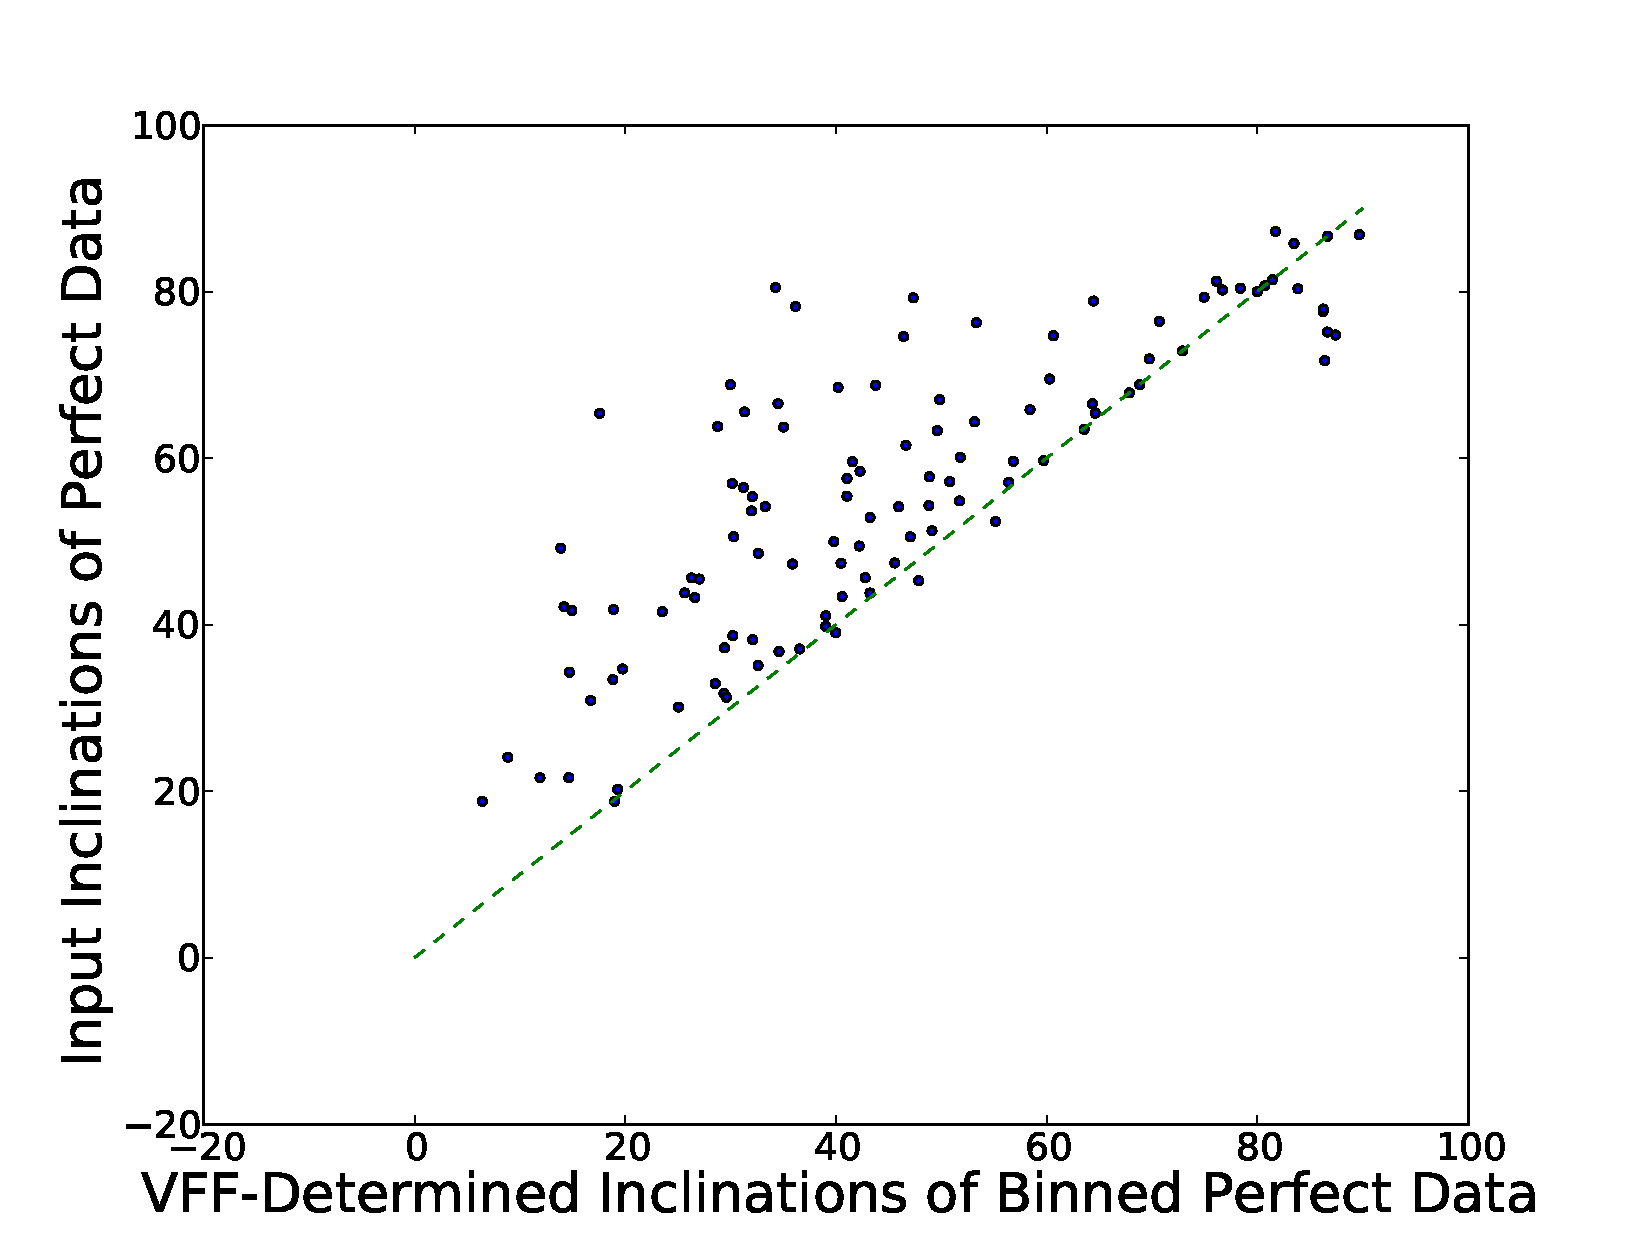
\includegraphics[width=0.5\textwidth]{binnedtest.pdf}
\caption{A comparison of the input inclinations and the inclinations determined from much more poorly sampled perfect velocity fields. \label{fig:test}}
\end{figure}

\subsection{Binned Down Turbulent Fields}
This is the ultimate test, and will determine if VFF does okay in the worst case possible, but most realistic. DO THIS TEST AND PLOT THE RESULTS!!!
%%%%%% WRITE FINDINGS FROM CHECKING THIS!!! %%%%%%%%%

\subsection{Real Data}

\begin{figure}[h]
\begin{center}
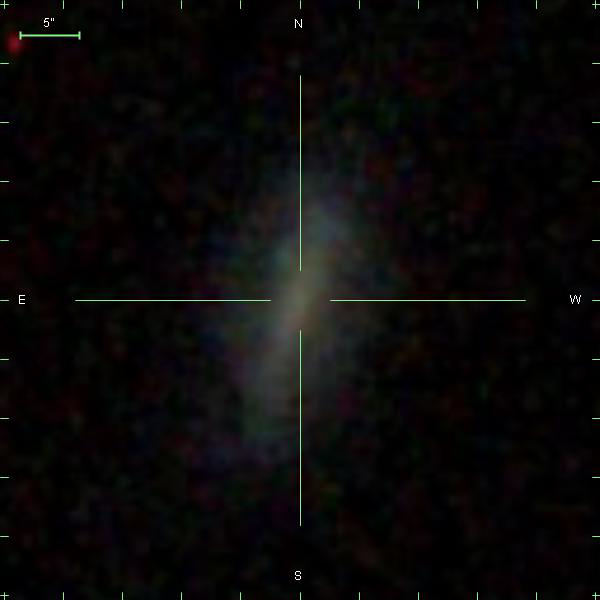
\includegraphics[width=0.34\textwidth]{tinygal.jpg}
\end{center}
\vspace{-0.4cm}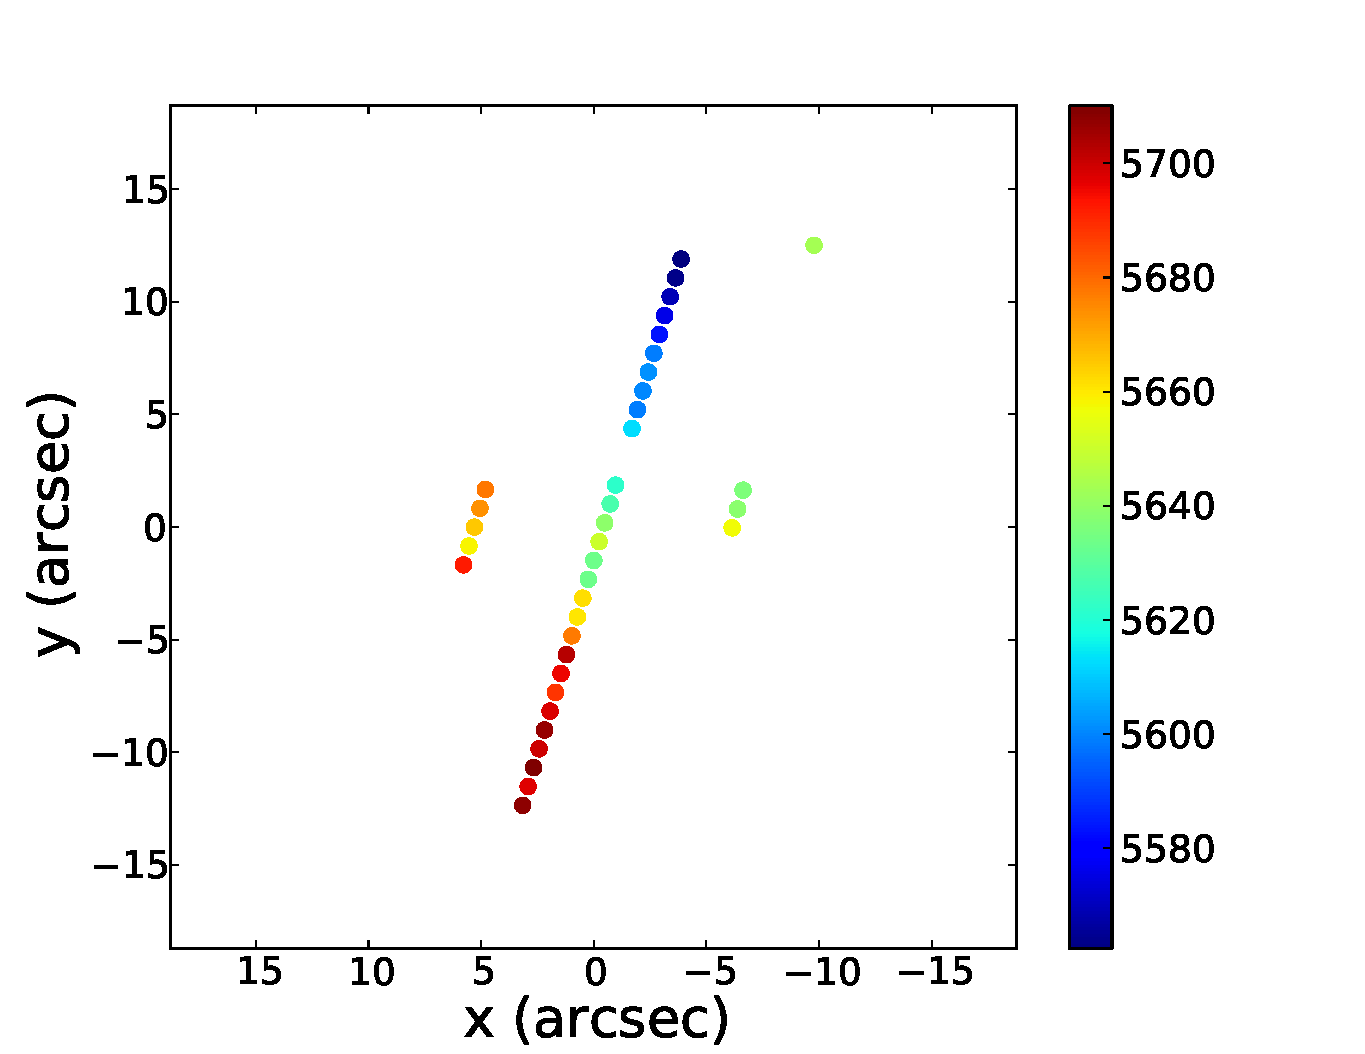
\includegraphics[width=0.5\textwidth]{rawvels.pdf}
\caption{The SDSS image and the SOAR spectrum of a galaxy in the survey. \label{fig:test}}
\end{figure}

With real data, VFF fits similarly to DiskFit, but with a larger degree of variance from the photometric counterparts. PRESENT AN ANALYSIS OF REAL DATA AND PHOTOMETRIC PROPERTIES TO BE DISCUSSED IN DISCUSSIONS AND CONCLUSIONS.
%%%%%% WRITE FINDINGS FROM CHECKING THIS!!! %%%%%%%%%


%---------------------------------------------------------------------------------%
%                               Section 5: Discussion                             %
%---------------------------------------------------------------------------------%

\section{Discussion}
%%%%%%%% FINISH!!!! %%%%%%%%
\section{Conclusions}
%%%%%%%% FINISH!!!! %%%%%%%%
\section{Acknowledgements}
%%%%%%%% FINISH!!!! %%%%%%%%
\newpage

\bibliographystyle{apj}
\bibliography{references}

%\section{Introduction}
%
%The introduction should contain sufficient
%background on the topic of your research that the reader understands what
%you are doing and why. It is important here and elsewhere in the paper to
%cite references when appropriate. While one can do this manually -- e.g
%(Vollbach et al. 1997), the easiest was to do this is with bibtex and the
%cite commands, because this automatically updates the references in both
%the text and the reference list at the end. For example, you can put the
%reference \cite{hamann2008}, or if you want it in line rather than in
%braces, then \citet{hamann2008}. To compile the documents you must then
%also have a .bib file (e.g. ast4723.bib) that contains the ADS bibtex entry, with
%the article name given as hamann2008, as in the example with this document.
%The document are then compiled by typing:
%
%bibtex ast4723
%latex ast4723.tex ; dvips -o ast4723.ps ast4723.dvi
%latex ast4723.tex ; dvips -o ast4723.ps ast4723.dvi
%
%Mote that you have to latex it twice after adding references for all the references
%to get updated.
%The following examples of sections are intended to provide a rough guideline for how
%you may wish to structure your paper. You are not required to maintain this format,
%but should use a similar, sensible approach.
%
%You may need to have emulateapj.cls in the same directory as your document.
%
%
%\section{Observations}
%
%In this section you should describe your observations. Look at a real paper (or
%at least the sample.tex file with emulateapj) to get an idea for what is appropriate
%in this section. Be sure to include information about what nights you observed
%and any key issues related to your data quality.  If you are using archival data,
%then you should describe when the data was originally obtained and still describe 
%things such as the instrument and telescope.
%
%\section{Data Reductions}
%
%This section is your chance to describe everything that you did to process your data.
%List clearly how you reduced the data and did the photometry. If you wish to divide
%this into subsections, you can do so as illustrated below.
%\subsection{Bias Subtraction and Flatfielding}
%To subtract the bias, we...
%\subsection{Really weird stuff that I had to do for my data}
%There was a bad region shaped like a parrot in the middle of the detector, which required...
%\subsection{Image Stacking}
%We aligned the images using...
%\subsection{Photometric Calibration}
%
%\section{Data Analysis}
%
%This section should describe the scientific analysis done for your project. If you are
%making a light curve for example, here is where you would describe how you made it and what you measured.
%Remember that your write-up should contain figures, such as Figure \ref{fig:test}. Note that this
%reference to the figure is collected to a label in the figure caption, so if you add others the
%number will automatically update
%
%\section{Results and Discussion (can easily be separate sections)}
%
%Fairly self explanatory. You should think carefully about what your results 
%mean. Speculation is good, but it should be grounded in the data -- wild
%speculation is bad.  If you want to add any equations in the text, this
%can be done in the fashion below. Note that the online latex references, 
%including the ones linked off the web page, provide the necessary information
%for constructing more complex equations. If you want to include equation
%symbols inline in the text, then you place them between dollar signs, as
%shown below.
%
%Consider the equation
%\begin{equation}
%\bar v = \exp(\tau^{-1})
%\end{equation}
%where $\bar v$ is the mean velocity of a purple balloon, and $\tau$ is
%the mean free path of the balloon. If we have a velocity $\bar v = 5\pm1$ km s$^{-1}$,
%what is $\tau$?
%
%One last item that we have not discussed is tables. There is an example in this
%document in Table \ref{tab:test}, which is the same as in sample.tex.
%
%\acknowledgments
%
%Anyone whom you would like to thank would go in this section (not required). 
%
%
%\appendix
%
%\section{Appendix material}
%
%If you want to go into a lot of detail about something that you feel doesn't belong
%in the main part of the paper, this would be the place to do it. 
%
%For this document, I will simply note that for the bibliographies, the manual
%way of including a bibliography is
%\begin{verbatim}
%\begin{thebibliography}{}
%\bibitem[Auri\`ere(1982)]{aur82} Auri\`ere, M.  1982, \aap,
%    109, 301
%\bibitem[Canizares et al.(1978)]{can78} Canizares, C. R.,
%    Grindlay, J. E., Hiltner, W. A., Liller, W., \&
%    McClintock, J. E.  1978, \apj, 224, 39
%\bibitem[Djorgovski \& King(1984)]{djo84} Djorgovski, S.,
%    \& King, I. R.  1984, \apjl, 277, L49
%\bibitem[Hagiwara \& Zeppenfeld(1986)]{hag86} Hagiwara, K., \&
%    Zeppenfeld, D.  1986, Nucl.Phys., 274, 1
%\bibitem[Harris \& van den Bergh(1984)]{har84} Harris, W. E.,
%    \& van den Bergh, S.  1984, \aj, 89, 1816
%\bibitem[King(1966)]{kin66}  King, I. R.  1966, \aj, 71, 276
%\bibitem[Ortolani et al.(1985)]{ort85} Ortolani, S., Rosino, L.,
%    \& Sandage, A.  1985, \aj, 90, 473
%\bibitem[Peterson(1976)]{pet76} Peterson, C. J.  1976, \aj, 81, 617
%\end{thebibliography}
%\end{verbatim}
%
%while the automated way, assuming that you have generated a .bib file is

%
%which for the file ast4723.bib and this tex file generates the reference list
%seen below. A nice aspect of this approach is that if you don't use a reference
%in the paper it automatically gets removed from the reference list at the end.
%The one additional file that you need to have for this approach is apj.bst,
%which is posted on the web page.
%
%
%\bibliographystyle{apj}
%\bibliography{references}
%
%\clearpage
%
%\begin{deluxetable}{ccrrrrrrrrcrl}
%\tabletypesize{\scriptsize}
%\tablecaption{Sample table taken from \citet{treu03}\label{tbl-1}}
%\tablewidth{0pt}
%\tablehead{
%\colhead{POS} & \colhead{chip} & \colhead{ID} & \colhead{X} & \colhead{Y} &
%\colhead{RA} & \colhead{DEC} & \colhead{IAU$\pm$ $\delta$ IAU} &
%\colhead{IAP1$\pm$ $\delta$ IAP1} & \colhead{IAP2 $\pm$ $\delta$ IAP2} &
%\colhead{star} & \colhead{E} & \colhead{Comment}
%}
%\startdata
%0 & 2 & 1 & 1370.99 & 57.35    &   6.651120 &  17.131149 & 21.344$\pm$0.006  & 2 4.385$\pm$0.016 & 23.528$\pm$0.013 & 0.0 & 9 & -    \\
%0 & 2 & 2 & 1476.62 & 8.03     &   6.651480 &  17.129572 & 21.641$\pm$0.005  & 2 3.141$\pm$0.007 & 22.007$\pm$0.004 & 0.0 & 9 & -    \\
%0 & 2 & 3 & 1079.62 & 28.92    &   6.652430 &  17.135000 & 23.953$\pm$0.030  & 2 4.890$\pm$0.023 & 24.240$\pm$0.023 & 0.0 & - & -    \\
%0 & 2 & 4 & 114.58  & 21.22    &   6.655560 &  17.148020 & 23.801$\pm$0.025  & 2 5.039$\pm$0.026 & 24.112$\pm$0.021 & 0.0 & - & -    \\
%0 & 2 & 5 & 46.78   & 19.46    &   6.655800 &  17.148932 & 23.012$\pm$0.012  & 2 3.924$\pm$0.012 & 23.282$\pm$0.011 & 0.0 & - & -    \\
%0 & 2 & 6 & 1441.84 & 16.16    &   6.651480 &  17.130072 & 24.393$\pm$0.045  & 2 6.099$\pm$0.062 & 25.119$\pm$0.049 & 0.0 & - & -    \\
%0 & 2 & 7 & 205.43  & 3.96     &   6.655520 &  17.146742 & 24.424$\pm$0.032  & 2 5.028$\pm$0.025 & 24.597$\pm$0.027 & 0.0 & - & -    \\
%0 & 2 & 8 & 1321.63 & 9.76     &   6.651950 &  17.131672 & 22.189$\pm$0.011  & 2 4.743$\pm$0.021 & 23.298$\pm$0.011 & 0.0 & 4 & edge \\
%\enddata 
%%% Text for table notes should follow after the \enddata but before %% the \end{deluxetable}. Make sure there is at least one \tablenotemark
%%% in the table for each \tablenotetext.  
%\tablecomments{Table \ref{tbl-1} is published in its entirety in the electronic edition of the {\it Astrophysical Journal}. A portion is shown here for guidance
%regarding its form and content.}
%
%\tablenotetext{a}{Sample footnote for table~\ref{tbl-1} that was generated
%with the deluxetable environment}
%\tablenotetext{b}{Another sample footnote for table~\ref{tbl-1}}
%
%\end{deluxetable}

\end{document}

%%
%% End of file `sample.tex'.
